\section{Modello del paziente}
L'organismo umano è un sistema molto complesso formato da molti sottosistemi interagenti fra loro altrettanto complessi, come ad esempio il sistema cardio-circolatorio, nervoso, respiratorio, digerente, \ldots
La dialisi è una procedura terapeutica che serve a ristabilire, per quanto possibile, un equilibrio chimico e volumetrico dell'organismo e, per questo motivo, verrà considerata solo quella parte dell'organismo direttamente coinvolta negli scambi di liquidi e soluti, ignorando tutto il resto.

Quello che è racchiuso in \figurename\ref{schema_generale} dalla linea tratteggiata grigia e recante l'etichetta ``\textsc{Paziente}'' rappresenta ciò che può essere considerato il paziente nel contesto dialitico: si tratta di un recipiente, formato da tre compartimenti sempre più profondi e capienti, separati da due membrane semipermeabili: la membrana capillare e la membrana cellulare. Questo schema è tratto da Guyton et al. \cite{guyton}. Nella realtà fisiologica, tuttavia, non esistono compartimenti e membrane così ben definiti. Nell'organismo umano infatti le cellule, e ciò che racchiudono, sono distribuite in maniera omogenea in tutto il volume corporeo; lo spazio interstiziale è un ambiente identificato topologicamente dal percorso che i metaboliti compiono per passare dall'apparato circolatorio alle cellule; il volume plasmatico è contenuto nelle arterie, vene e capillari dell'organismo. Per le mebrane cellulari e capillari il discorso è analogo: esistono numerose membrane di ambo i tipi sparse omogeneamente all'interno del volume corporeo. Per semplificare la trattazione matematica si è deciso di semplificare il problema andando a ``concentrare'' i volumi cellulari, interstiziali ed ematici, distribuiti nell'organismo, in tre compartimenti nettamente divisi dalle membrane appropriate: la topologia degli scambi di massa e volume, nonostante questa azzardata semplificazione, resta inalterata.

\subsection{Bilancio di massa nel compartimento intra-cellulare}
L'equazione che descrive il bilancio di massa per il soluto $(s)$ all'interno del compartimento intracellulare è:
\begin{equation}
	\frac{dM_{ic}^{(s)}}{dt} = G_{ic}^{(s)}+ \Phi_{ic}^{(s)}
	\label{eq:dMic}
\end{equation}
dove:
\begin{itemize}
	\item $G_{ic}^{(s)}$ è il tasso di generazione del soluto $(s)$ all'interno delle cellule;
	\item $\Phi_{ic}^{(s)}$ è il flusso di massa del soluto $(s)$ verso l'interno del compartimente intracellulare.
\end{itemize}
\begin{figure}[htb]
	\centering
		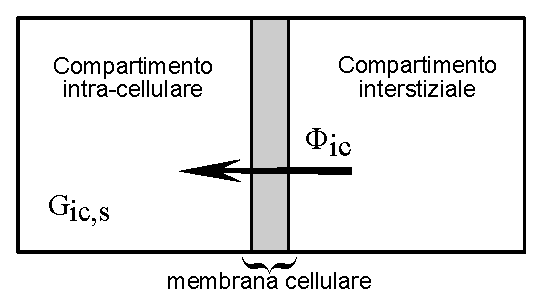
\includegraphics[width=0.5\textwidth]{immagini/massa_ic.eps}
				\caption{Scambio di soluto nel compartimento cellulare.}
\end{figure}
La formula per $\Phi_{ic}^{(s)}$ è data dall'equazione (\ref{flusso_ic}) e cioè:
\begin{equation}
	\Phi_{ic}^{(s)} = - k^{(s)} \bigl(C_{ic}^{(s)} - \beta^{(s)} C_{is}^{(s)}\bigr)
	\label{eq:phi_ic}
\end{equation}
in cui, come già spiegato in \textsection\ref{trasp_cel}:
\begin{itemize}
	\item $k^{(s)}$ è il coefficiente di trasferimento di massa per il soluto $(s)$, proporzionale alla velocità del processo di scambio fra spazio interstiziale e intracellulare;
	\item $\beta^{(s)}$ è il rapporto all'equilibrio fra concentrazione intracellulare $C_{ic}^{(s)}$ e interstiziale $C_{is}^{(s)}$ del soluto $(s)$.
\end{itemize}
La concentrazione del soluto $(s)$ può essere espressa in funzione della sua quantità e del volume in cui è distribuito. Per quanto riguarda il compartimento intracellulare, vale ovviamente:
\begin{equation}\label{eq:ovvia}
	C_{ic}^{(s)} = \frac{M_{ic}^{(s)}}{V_{ic}}
\end{equation}
Se si considera l'effetto Donnan (\textsection\ref{sec:donnan}), si può scrivere la concentrazione interstiziale in funzione di quella plasmatica, ovvero:
\begin{equation}
	C_{is}^{(s)} = \alpha_d^{(s)}\cdot C_{pl}^{(s)}
	\label{eq:donnfrac}
\end{equation}
in cui $\alpha_d^{(s)}$ è il coefficiente di Donnan per il soluto $(s)$, il cui calcolo è esposto in Appendice \ref{app:A}.
Ora, poiché il compartimento extracellulare è formato dal compartimento interstiziale più quello plasmatico, per la conservazione della massa vale che:
\begin{align*}
	M_{ex}^{(s)} &= M_{is}^{(s)} + M_{pl}^{(s)} \\
	             &= C_{is}^{(s)} V_{is} + C_{pl}^{(s)} V_{pl}
\end{align*}
e considerando l'equazione (\ref{eq:donnfrac}) è possibile scrivere:
\begin{equation}\label{eq:meno_ovvia}
	M_{ex}^{(s)} = C_{is}^{(s)} V_{is} + \frac{C_{is}^{(s)}}{\alpha_d^{(s)}} V_{pl}
\end{equation}
da cui si ricava:
\begin{equation*}
	C_{is}^{(s)} = \frac{M_{ex}^{(s)}}{V_{is} + V_{pl}/\alpha_d^{(s)}}
\end{equation*}
A questo punto, considerando nullo il tasso di generazione intracellulare del soluto,si può riscrivere l'equazione (\ref{eq:dMic}) nel seguente modo:
\begin{equation}
	\frac{dM_{ic}^{(s)}}{dt} = - k^{(s)} \biggl(\frac{M_{ic}^{(s)}}{V_{ic}} - \beta^{(s)} \frac{M_{ex}^{(s)}}{V_{is} + V_{pl}/\alpha_d^{(s)}}\biggr)
\end{equation}

\subsection{Bilancio di massa nel compartimento extra-cellulare}
Il bilancio di massa nel compartimento extra-cellulare tiene conto dei flussi di soluto attraverso la membrana capillare e attraverso la membrana del dializzatore, e si tratta di flussi di perdita e quindi negativi, in formule:
\begin{equation}
	\frac{dM_{ex}^{(s)}}{dt} = -\Phi_{ic}^{(s)} -\Phi_{hdf}^{(s)} + Q_s\cdot C_s^{(s)}
\end{equation}
in cui:
\begin{itemize}
	\item $Q_s$ è la portata del fluido di sostituzione (ovvero la portata di pre- o post-diluizione), letta sul monitor della macchina;
	\item $C_s^{(s)}$ è la concentrazione del soluto $(s)$ nel liquido di sostituzione, calcolata con l'Eq.(\ref{eq:liquido});
	\item $\Phi_{ic}^{(s)}$ è data dall'equazione (\ref{eq:phi_ic}),
	\item $\Phi_{hdf}^{(s)}$ è calcolata con l'Eq.(\ref{phihdf}).	
\end{itemize}
\begin{figure}[htb]
	\centering
		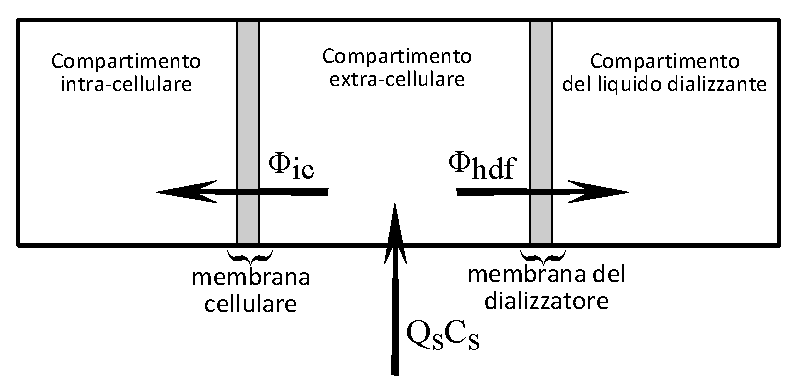
\includegraphics[width=0.8\textwidth]{immagini/massa_ex.eps}
				\caption{Scambio di soluto nel compartimento extracellulare.}
\end{figure}
Vale la pena precisare ancora il calcolo di $\Phi_{hdf}^{(s)}$. Dalla teoria esposta in \textsection\ref{sec:HDF}, risulta:
\begin{multline}\label{eq:phihdf}
		\qquad \Phi_{hdf}^{(s)} = (1-FF)\cdot \biggl[D^{(s)}\biggl(\alpha_d^{(s)} C_{in}^{(s)} - C_d^{(s)}\biggr)+\Phi_t^{(s)} \biggr] + \ldots \\
		                 + FF\cdot \biggl[Q_{in}-(1-\eta^{(s)})Q_f\biggr] C_{in}^{(s)} \qquad
\end{multline}
col termine convettivo pari a:
\begin{equation*}
	\Phi_t^{(s)} = Q_f \bigl(1-\sigma^{(s)}\bigr) \frac{C_{in}^{(s)} + C_d^{(s)}}{2}
\end{equation*}
Si ricordi che $FF$ è la frazione di filtrazione, pari al rapporto $Q_f/Q_{in}$ fra acqua filtrata e acqua in ingresso al dializzatore. Il calcolo dei coefficienti $D^{(s)}$, $\alpha_d^{(s)}$, $\sigma^{(s)}$ è affrontato in Appendice \ref{app:B}. I valori di concentrazione $C_d^{(s)}$ dei soluti nel liquido di dialisi, sono forniti dall'Eq.(\ref{eq:liquido}).

\subsection{Bilancio volumetrico nel compartimento intracellulare}
La variazione nel tempo del volume intracellulare, dipende, attraverso il coefficiente $K_f$ (permeabilità della membrana cellulare all'acqua), dalla differenza osmotica fra spazio intracellulare e spazio interstiziale. In formule:
\begin{equation}\label{eq:vicnot}
	\begin{split}
	\frac{dV_{ic}}{dt} &= Q_{ic}\\
										 &= \gamma K_f \cdot \Delta Osm \\
	                   &= \gamma K_f \sum_j{\sigma_j\biggl(C_{ic}^{(j)}-C_{is}^{(j)}\biggr)}
	\end{split}
\end{equation}
\begin{figure}[htb]
	\centering
		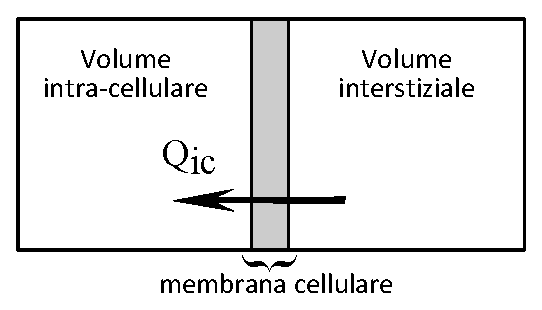
\includegraphics[width=0.5\textwidth]{immagini/vol_ic.eps}
				\caption{Scambio di fluido nel volume cellulare.}
\end{figure}
in cui $\gamma=0,93$ è il coefficiente di correzione che tiene conto dell'interazione osmotica fra i soluti, e $\sigma_j$ è il coefficiente di riflessione della membrana cellulare nei confronti del soluto $j$ (ricordiamo che l'effetto osmotico è dovuto ai soluti che \textit{non} passano la membrana).
In condizioni di equilibrio, e cioè qualora sostituissimo alle concentrazioni intracellulari e interstiziali dell'Eq.(\ref{eq:vicnot}) gli opportuni valori ricavati dalla \tablename~\ref{tab:osmolarit} in Appendice \ref{app:A}, si dovrebbe ottenere, per definizione di ``condizione di equilibrio'', che la variazione temporale del volume intracellulare si annulli. Così come è scritta, l'Eq.(\ref{eq:vicnot}) non soddisfa questa condizione. Ciò è dovuto al fatto di non aver considerato, nella sommatoria, tutti i soluti presenti nell’organismo, solo parte dei quali è tabulata in \tablename~\ref{tab:osmolarit}. Ovviamente è impossibile, data la loro numerosità, considerarli tutti. Ciò non toglie che comunque, nel calcolo dei flussi osmotici, si generi
involontariamente un disequilibrio causato dai soluti mancanti all’appello. Per risolvere questo problema si è pensato, utilizzando un approccio \textit{teleologico}
\footnote{\textit{`` [\ldots] in fisiologia la dottrina teleologica risulta indubbiamente utile; anche se è ufficialmente respinta, i pericoli che comporta la sua adozione sono assai modesti [\ldots] ''}.Tratto da A.~C.~Burton, Fisiologia e Biofisica della Circolazione.}, di ipotizzare quanto segue. 
Quando si prendono in considerazione i soluti che interessa analizzare, indipendentemente dalla loro numerosità, ci saranno sempre degli altri soluti, esclusi dal calcolo, che \textit{all'equilibrio} (ovvero \textit{asintoticamente}) ne bilanceranno l'attività osmotica in quantità pari in modulo a quella dei soluti inclusi nel calcolo. In altre parole, nel momento in cui i soluti di interesse raggiungeranno lo stato di equilibrio potremmo ipotizzare che quelli esclusi dal calcolo siano distribuiti in maniera tale che il sistema smetta di evolvere.
\newline
\indent
A questo punto, è doveroso fare un breve \textit{excursus} per precisare cosa intendiamo, quantitativamente, per ``stato di equilibrio'' In questa trattazione abbiamo deciso di usare, come stato di equilibrio, quello stato, calcolato ad ogni iterazione, in cui le concentrazioni plasmatiche, interstiziali e intracellulari, abbiano fra loro \textit{gli stessi rapporti numerici} di quelli di \tablename~\ref{tab:osmolarit}. Analogamente, definiamo i \textit{volumi di equilibrio} quei volumi plasmatici, interstiziali e intracellulari, che hanno fra loro \textit{gli stessi rapporti numerici} di quelli in \tablename~\ref{tab:volumi_guyton}. Precisiamo che queste quantità di equilibrio, che il sistema asintoticamente tende a raggiungere, devono essere ricalcolate ad ogni iterazione.

Per ricavare i volumi asintotici di equilibrio, ad ogni iterazione si eseguirà il seguente algoritmo di calcolo:
\begin{align}
		V_{tot,\infty}      &= V_{ic}+V_{is}+V_{pl}   \qquad \text{con $V_{ic}$, $V_{is}$, $V_{pl}$, valori correnti}\\
		V_{pl,\infty}       &= 3/42  \cdot V_{tot,\infty} \\
		V_{is,\infty}       &= 11/42 \cdot V_{tot,\infty} \\
		V_{ic,\infty}       &= 28/42 \cdot V_{tot,\infty} \\
\end{align}
Per ricavare le concentrazioni asintotiche:
\begin{align*}
		M_{tot,\infty}^{(s)} &= M_{ic}^{(s)}+M_{ex}^{(s)} \qquad\qquad \text{con $M_{ic}$, $M_{ex}$, valori correnti}\\
		                     &= V_{pl,\infty}\cdot C_{pl,\infty}^{(s)} + V_{is,\infty}\cdot C_{is,\infty}^{(s)}  + V_{ic,\infty}\cdot C_{ic,\infty}^{(s)} \\
		                     &= V_{pl,\infty}\cdot C_{pl,\infty}^{(s)} + V_{is,\infty}\cdot\alpha^{(s)}C_{pl,\infty}^{(s)}  + V_{ic,\infty}\cdot\alpha^{(s)}\beta^{(s)}C_{pl,\infty}^{(s)}   \\
		                     &= C_{pl,\infty}^{(s)} \biggl(V_{pl,\infty} + \alpha^{(s)}\bigl(V_{is,\infty} + \beta^{(s)}V_{ic,\infty}\bigr)\biggr)
\end{align*}
da cui si ricava:
\begin{align}
		C_{pl,\infty}^{(s)} &= \frac{M_{ic}^{(s)}+M_{ex}^{(s)}}{V_{pl,\infty} + \alpha^{(s)}\bigl(V_{is,\infty} + \beta^{(s)}V_{ic,\infty}\bigr)} \\
		C_{is,\infty}^{(s)} &= \alpha^{(s)} C_{pl,\infty}^{(s)} \\
		C_{ic,\infty}^{(s)} &= \beta^{(s)}  C_{is,\infty}^{(s)} 
\end{align}
\newline
\indent
Tornando ora ad occuparsi dell'equazione che descrive la variazione del volume intracellulare. Alla luce di tutte le considerazioni fatte sin ora, è possibile costruire il termine \textit{differenza osmotica asintotica} nel seguente modo:
\begin{equation}
	\Delta Osm_{\infty} = \sum_j{\sigma_j\bigl(C_{ic,\infty}^{(j)}-C_{is,\infty}^{(j)}\bigr)}
\end{equation}
Affinché l'Eq.(\ref{eq:vicnot}), con la quale si è partiti, possa soddisfare la condizione che una volta inseriti valori di equilibrio la derivata temporale si annulli in un tempo finito, deve essere modificata e assumere la seguente forma:
\begin{equation}\label{eq:vicyes}
	\begin{split}
	\frac{dV_{ic}}{dt} &= Q_{ic}\\
										 &= \gamma K_f \bigl(\Delta Osm - \Delta Osm_{\infty}\bigr)
	\end{split}										 
\end{equation}
che esplicitata diventa:
\begin{equation*}
	\frac{dV_{ic}}{dt} = \gamma K_f \biggl(\sum_j{\sigma_j\bigl(C_{ic}^{(j)}-C_{is}^{(j)}\bigr)} - \sum_j{\sigma_j\bigl(C_{ic,\infty}^{(j)}-C_{is,\infty}^{(j)}\bigr)}\biggr)
\end{equation*}

\subsection{Bilancio volumetrico nel compartimento interstiziale}
La variazione nel tempo del volume interstiziale, dipende sia dalla portata $Q_{ic}$ di liquido che dall'interstizio passa nel compartimento intracellulare, sia dalla portata $Q_{fc}$ di liquido che filtra, attraverso le pareti capillari, dal compartimento plasmatico. Quantitativamente:
\begin{equation}
	\frac{dV_{is}}{dt} = - Q_{ic} + Q_{fc}
\end{equation}
\begin{figure}[htb]
	\centering
		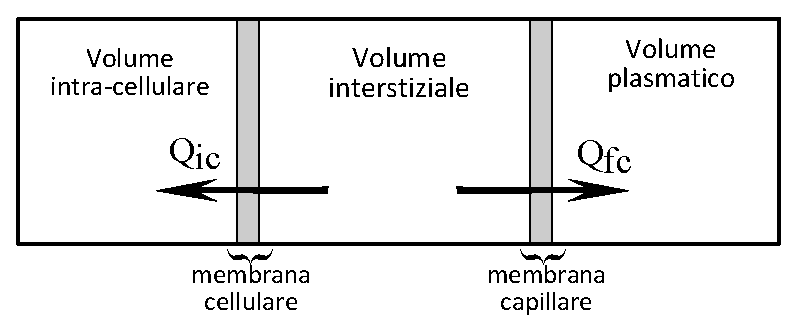
\includegraphics[width=0.8\textwidth]{immagini/vol_is.eps}
				\caption{Scambio di fluido nel volume interstiziale.}
\end{figure}
la portata $Q_{ic}$ si ricava dall'Eq.(\ref{eq:vicyes}). Per quanto riguarda la portata di filtrazione capillare, essa dipende dalla permeabilità della membrana capillare e dalla differenza di pressione cui è sottoposta. In formule:
\begin{equation}\label{eq:qfcnot}
	Q_{fc} = \rho(L_a+L_v)\cdot P_{fc}
\end{equation}
I parametri $L_a$ e $L_v$ rappresentano rispettivamente le permeabilità nella zona arteriosa e venosa della membrana capillare\footnote{questi elementi sono in parallelo fra loro e, poiché la premeabilità idraulica è analoga alla conduttanza elettrica, la premeabilità/conduttanza totale di due elementi posti in parallelo è data dalla somma delle singole permeabilità/conduttanze.}; il parametro adimensionale $\rho$ serve a dare variabilità alla permeabilità dei capillari, in quanto questa varia da paziente a paziente (diabete, stato infiammatorio, \ldots).
La pressione di filtrazione $P_{fc}$ dipende dalla pressione idraulica media nel letto capillare, dalla pressione idraulica dell'interstizio, e dalla differenza di pressione oncotica fra plasma e interstizio, cioè:
\begin{equation}
	P_{fc} = \biggl(\frac{P_{ac}+P_{vc}}{2} - P_{is}\biggr) - \Delta \Pi
\end{equation}
in cui la differenza di pressione oncotica $\Delta \Pi$ è calcolata con la formula di Landis-Pappenheimer in base alla concentrazione proteica dei rispettivi compartimenti. Le pressioni idrauliche si calcolano a partire dai volumi, attraverso i valori di \textit{compliance} o \textit{elastanza} dei compartimenti:
\begin{align}
  P_{is} &= E_{is} (V_{is}-V_{is,0}) + P_{is,0} \qquad \text{con $E_{is}=$ elastanza dell'interstizio}\\
	P_{ac} &= \frac{1}{Cc} (V_{pl}-V_{pl,0}) + P_{is,0} \qquad \text{con $C_c=$ compliance capillare} \\
	P_{vc} &= 15\text{ mmHg} \qquad \text{costante}
\end{align}

Se ora si dà nuovamente uno sguardo al riquadro ``paziente'' di \figurename\ref{schema_generale}, si nota che è stato tralasciato un importante dettaglio di bilancio fra plasma e interstizio: il sistema linfatico. Il sistema linfatico, quando non è compromesso da particolari patologie, svolge l'importante funzione di regolare il bilancio volumetrico fra plasma e interstizio favorendo, ad esempio, lo spostamento di liquidi e proteine dall'interstizio al plasma in caso di edema interstiziale \cite{guyton}. Per tenere in considerazione anche il sistema linfatico si utilizzerà anche in questo caso, per semplicità, un approccio teleologico. L'ipotesi operativa è che la funzione del sistema linfatico sia identificata da una pressione \textit{efficace}, che bilancia la pressione di filtrazione capillare $P_{fc}$. Questa pressione efficace, la si ipotizza pari in modulo alla pressione di filtrazione capillare calcolata utilizzando i valori asintotici di equilibrio, cioè:
\begin{equation}
	P_{fc,\infty} = \biggl(\frac{1/C_c\cdot V_{pl,\infty} + P_{vc}}{2} - E_{is}\cdot V_{is,\infty}\biggr) - \Delta \Pi_{\infty}
\end{equation}
Con quanto appena esposto, l'Eq.(\ref{eq:qfcnot}) diventa:
\begin{equation}\label{eq:qfcyes}
	Q_{fc} =  \rho \bigl(L_a+L_v\bigr)\cdot \bigl(P_{fc}-P_{fc,\infty}\bigr)
\end{equation}
ed effettuando le sostituizioni opportune, la variazione nel tempo del volume interstiziale è descritta dall'equazione:
\begin{equation}\label{eq:dVis}
	\frac{dV_{is}}{dt} = - \gamma K_f \bigl(\Delta Osm - \Delta Osm_{\infty}\bigr) + \rho \bigl(L_a+L_v\bigr)\cdot \bigl(P_{fc}-P_{fc,\infty}\bigr)
\end{equation}


\subsection{Bilancio volumetrico nel compartimento plasmatico}
La variazione nel tempo del volume plasmatico è descritta dall'equazione:
\begin{equation}\label{eq:dVpl}
	\frac{dV_{pl}}{dt} = -Q_{fc} - Q_{uf}
\end{equation}
\begin{figure}[htb]
	\centering
		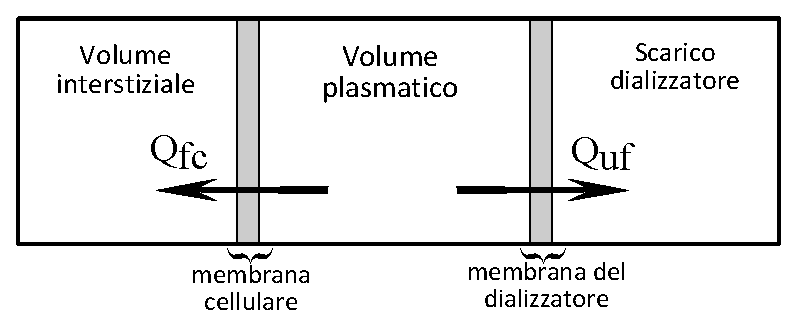
\includegraphics[width=0.8\textwidth]{immagini/vol_dia.eps}
				\caption{Scambio di fluido nel volume plasmatico.}
\end{figure}
in cui $Q_{fc}$ è dato dall'Eq.(\ref{eq:qfcyes}), e $Q_{uf}$ è la portata di ultrafiltrazione, cioè la portata che permette la perdita di peso del paziente durante la seduta dialitica. Bisogna fare attenzione a non confondere la portata di ultrafiltrazione con la portata di filtrazione del filtro dializzatore. Quest'ultima è infatti data dalla somma di ultrafiltrazione e portata di diluizione. Nell'Eq.(\ref{eq:dVpl}) infatti non compare la portata di diluizione proprio perché tutto il liquido di diluizione immesso nel circuito ematico, viene filtrato dal dializzatore.